%
% TU/e Style Master Thesis template for LaTeX
%
% Public version 1.0
% 2010 - 2013 Thijs Nugteren and Joos Buijs
%
% THIS IS THE MAIN FILE (i.e. compile this file, compiling the others directly won't work)
%
\documentclass[a4paper,10pt,twoside]{report}

%all the other includes etc. are done in the thesis.sty file.
\usepackage{thesis}

%
% These commands need to be defined in order to produce a correct and personalized document
%
\newcommand{\shortdoctitle}{TODO short title}
\newcommand{\doctitle}{TODO title}
\newcommand{\docsubtitle}{TODO subtitle}

\newcommand{\me}{Kelong Cong}
\newcommand{\keywords}{consensus, byzantine, blockchain}
\newcommand{\version}{Version 1.0}
\newcommand{\monthYear}{Month 2017}

%Be sure to use all the titles for your committee members!!! (their names show up on the very first page!)
\newcommand{\firstCommitteeMember}{Dr. J. Pouwelse}
\newcommand{\secondCommitteeMember}{Dr. Unknown}
\newcommand{\thirdCommitteeMember}{Prof. Unknown}

\author{\me}

%
% PDF settings
%
\hypersetup
{
    pdfauthor={\me},
    pdftitle={\shortdoctitle},
    pdfsubject={\doctitle},
    pdfkeywords={\keywords}
}

\begin{document}

%use this include for PDF and distribution versions
\pagenumbering{roman}
\begin{titlepage}
\begin{center}

\includegraphics[height=4cm]{figures/logo}\\
%\LARGE
%Delft University of Technology \\
\large
Faculty Electrical Engineering, Mathematics and Computer Science

\vspace*{12cm}

\setlength{\TPHorizModule}{1mm}
\setlength{\TPVertModule}{\TPHorizModule}
% Set the Paragraph Indent to zero, so the first line is not Indented
% Back-up the current value so it can be put back at the end of the title page
\newlength{\backupparindent}
\setlength{\backupparindent}{\parindent}
\setlength{\parindent}{0mm}			
% Begins a textbox at 72 mm from the left of the edge of the paper and 89 mm from the top
% The width of the textbox is 95 mm (167 - 72 mm)
% The height of the box cannot be defined, so it is your task to keep the text not too long
\begin{textblock}{95}(62,89)
    \vspace*{7mm}
    \huge
    \textbf{\doctitle \\}
    \Large
    \vspace*{3mm}
    \textit{\docsubtitle}\\
    \vspace*{10mm}
    \Large
    \me\\
\end{textblock}

\large
Supervisors:\\
\begin{tabular}{rl}
    \firstCommitteeMember\\
    \secondCommitteeMember\\
    \thirdCommitteeMember\\
\end{tabular}

\vfill
\version

\vfill
%\docdate \\
\large
Delft, \monthYear\\

% Put the Paragraph Indent back to its original value
\setlength{\parindent}{\backupparindent}
\end{center}
\end{titlepage} 


\normalsize

\clearemptydoublepage

%Sometimes line numbers are nice, uncomment the next line to enable:
%\linenumbers

%It could be handy to have a list of todos and brainstorms in your thesis
%\chapter*{*General todos*}\todo{remove this chapter}
%\input{chapters/general_todos}

%\chapter*{*Brainstorm results*}\todo{remove this chapter}
%\input{chapters/brainstorm_results}

\chapter*{Abstract}\label{chapter:abstract}
THIS IS MY ABSTRACT

\clearemptydoublepage

%An executive summary if you want:
%\chapter*{Executive summary}\label{chapter:executive_summary}
%\input{chapters/executive_summary}

%\clearemptydoublepage


\chapter*{Preface}\label{chapter:preface}
Please write all your preface text here. If you do so, don't forget to thank your supervisor, other committee members, your family, colleagues etc.\ etc. 

\clearemptydoublepage

\tableofcontents

%\clearemptydoublepage
%
%\listoffigures
%
%\clearemptydoublepage
%
%\listoftables
%
%\clearemptydoublepage
%
%\lstlistoflistings

\clearemptydoublepage

\chapter{Introduction}\label{chapter:intro}
\setcounter{page}{0}
\pagenumbering{arabic}
%from here on, start the 'real' page numbering, from 1, with normal digits
This is a story about a scalable blockchain framework and Byzantine
generals\dots

%%% Local Variables:
%%% mode: latex
%%% TeX-master: "../thesis"
%%% End:

\clearemptydoublepage

\chapter{Bottom-up Consensus}\label{chapter:consensus}
\section{Requirements}
\begin{itemize}
\item Permissionless
\item Byzantine fault tolerant
\item No PoW
\item Works under churn
\item Underlying data structure is TrustChain
\item Detects forks or double-spends
\item No step in the protocol blocks transactions
\item Application independent
\end{itemize}

\section{Assumptions}
\begin{itemize}
\item The total number of valiators is $N$. The number of faulty validators is
  no more than $f$, where $n > 3f$ (this value depends on BFT consensus
  algorithm that we use).
\item Validators have the complete history of the previously agreed set of
  transactions.
% \item Single connected component for TrustChain.
% \item No sybil attack % 
\item Weak synchrony, where messages are guaranteed to be delivered after
  $\Delta$ (also depends on BFT consensus algorithm). 
% TODO this depends on the BFT protocol and the broadcast protocol
% \item Rough (inaccurate to some degree) global clock
\end{itemize}

\section{Protocol}
The goal of the bottom-up consensus protocol is to validate a set of new
transactions against the previously validated transactions, and then disseminate
these transactions. For a set of transactions to be valid, they need to adhere
to the TrustChain construction. Out solution addresses the issue of Proof of Work
(wasteful) and classical BFT algorithms (does not scale).

To describe the protocol, we make two assumptions, later we show to these
assumptions are removed.
\begin{enumerate}
\item We assume there exist a set of validator nodes for every consensus run and
  for every round in a consensus run that are selected in a fair way and is
  known to all nodes. We address this assumption in \cref{sec:consensus-group}
  and \cref{sec:validator-group}.
\item We assume there exist a set of valid transactions from the previous
  consensus run. Every node knows the Merkle hash of this set of transactions.
  Assumption addressed in \cref{sec:bootstrapping}.
\end{enumerate}
\Cref{fig:protocol-init} shows the state of the system. Before explaining the
four phases of the protocol, we describe the concept of checkpointing.

\begin{figure}[htb]
	\centering
	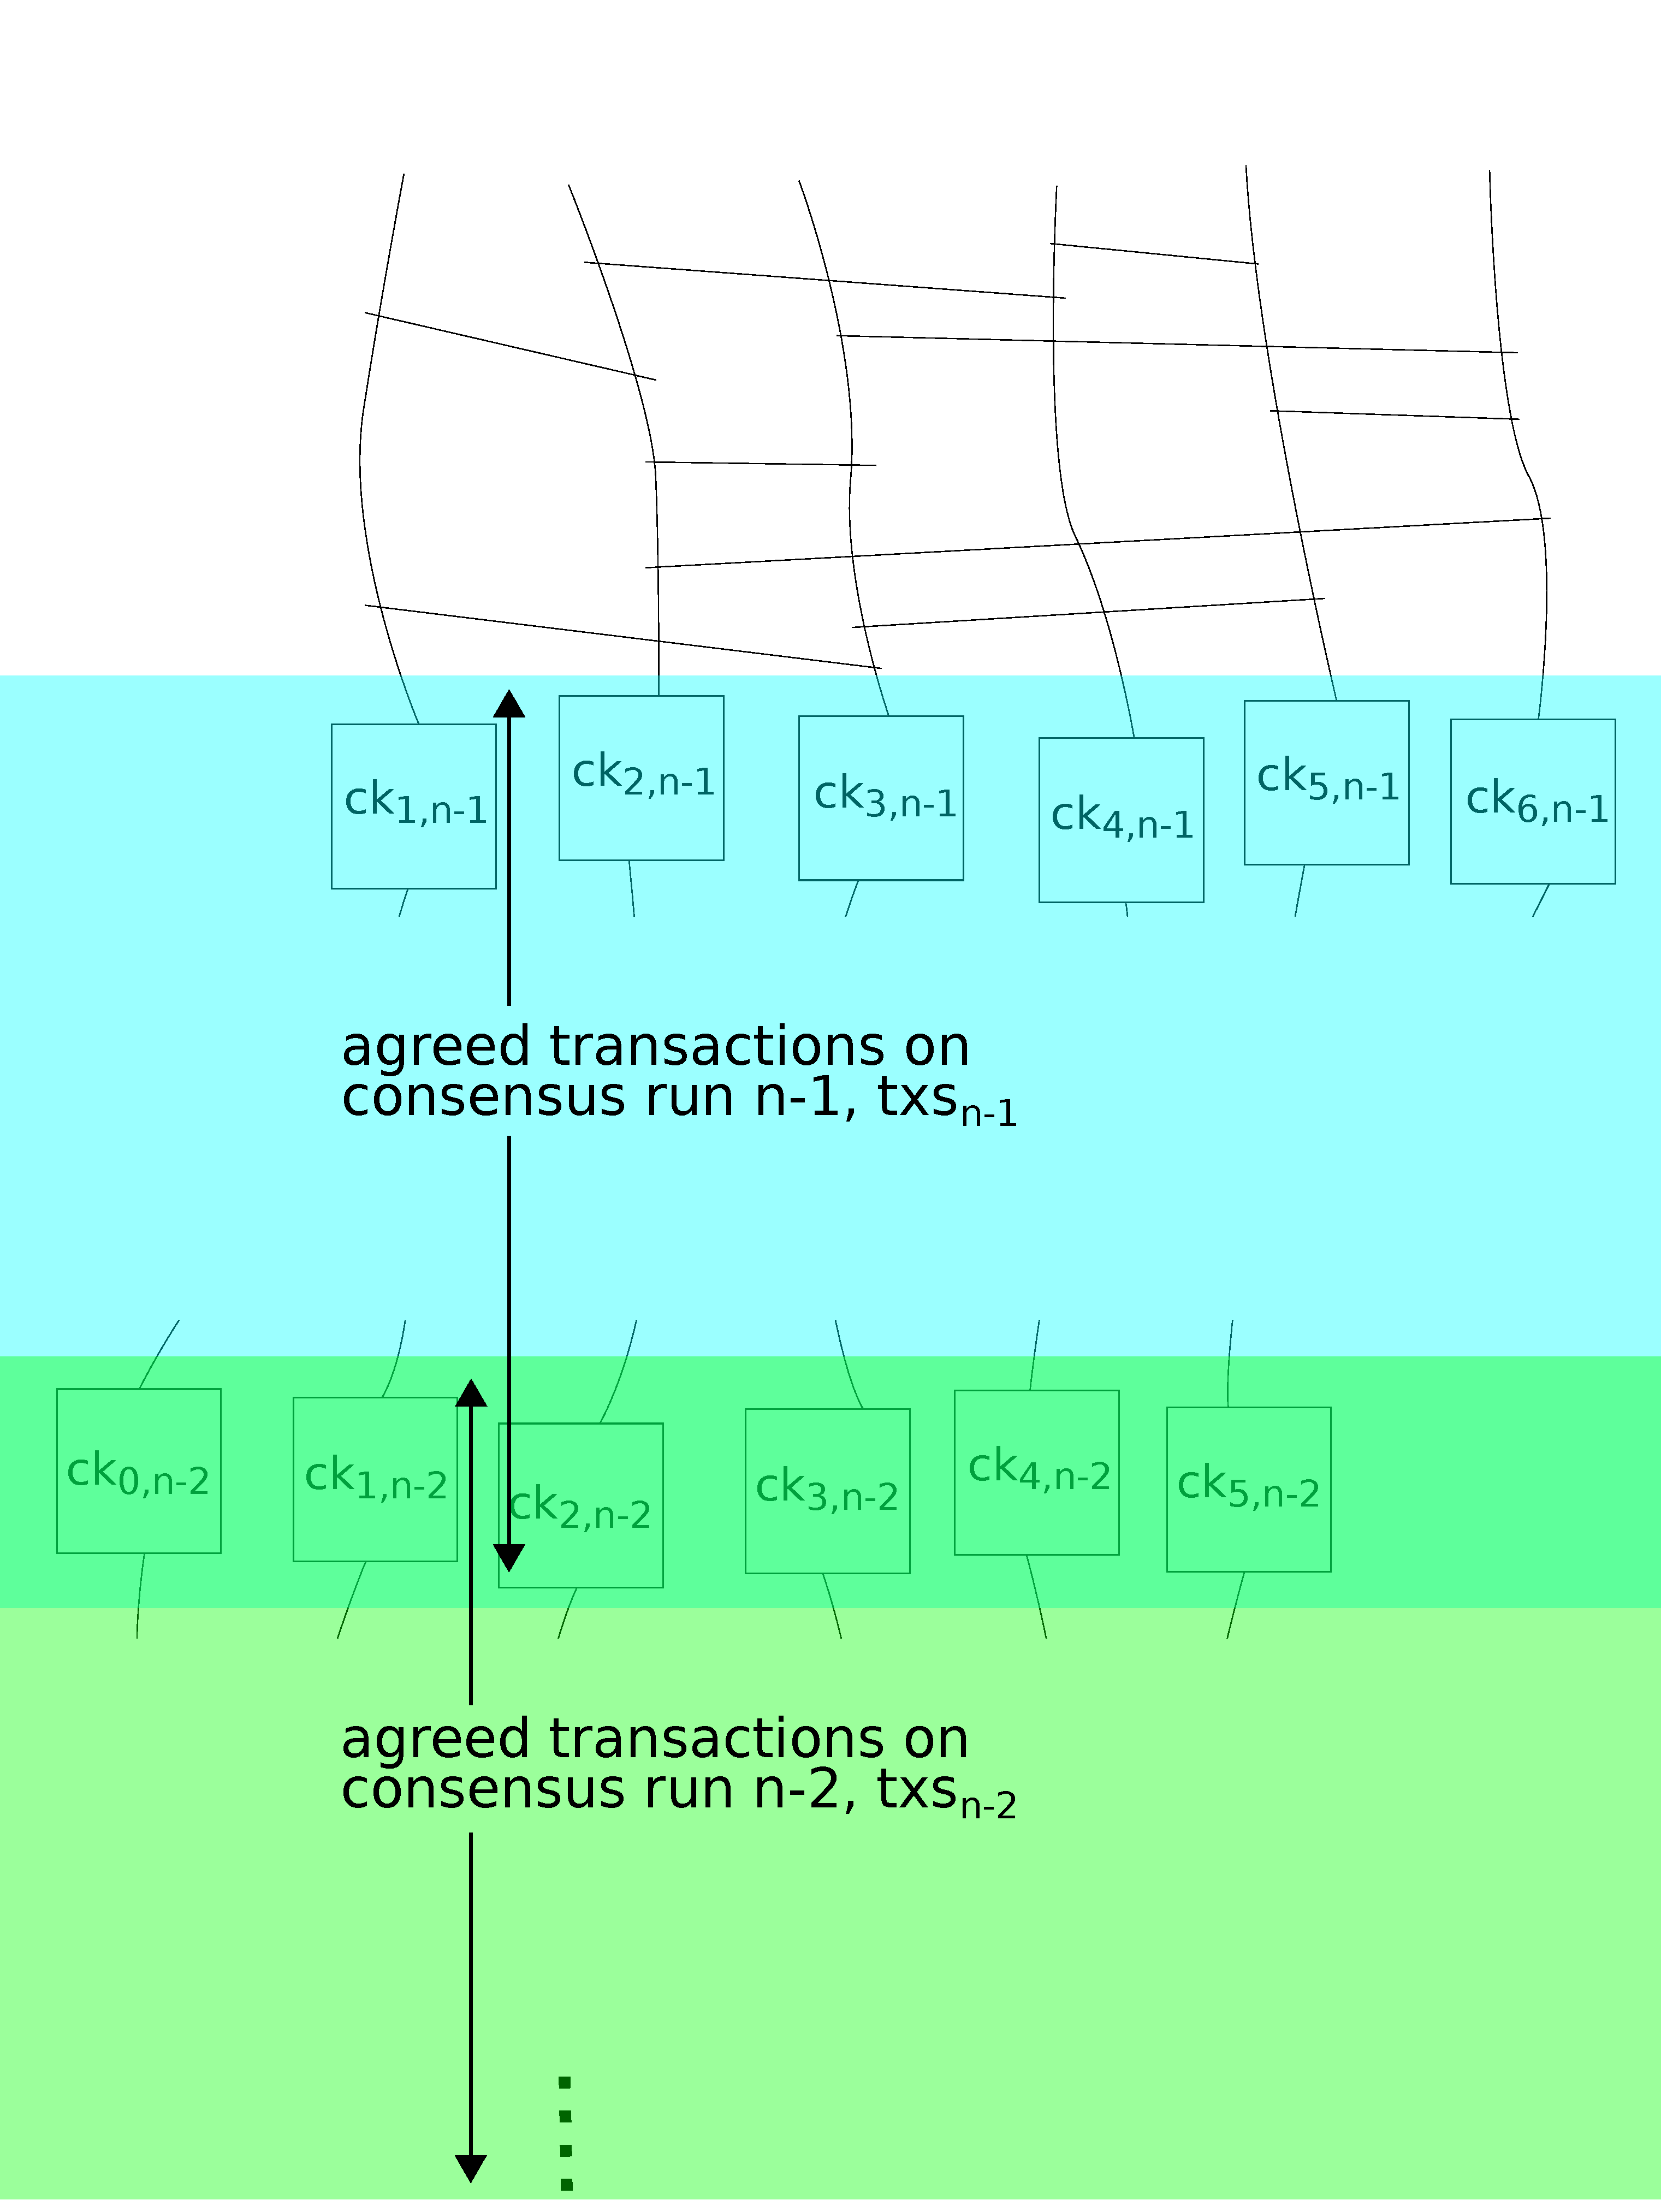
\includegraphics[width=0.7\textwidth]{figures/protocol-init}
	\caption{The initial state of the bottom-up consensus protocol. The thin
      lines are hash pointers to transactions and $ck_{x,n}$ represents a
      checkpoint block, where $x$ is the node ID and $n$ is the consensus run.}
    \label{fig:protocol-init}
\end{figure}

\subsection{Checkpointing}
A checkpoint block is a self-transaction where its input and output only involve
the node itself. Node $x$ creates the checkpoint block using
$$
ck_{x,n} = H(pk_x || H(txs_{n-1})),
$$
where $H$ is a cryptographically secure hash function, $pk_{x}$ is public key of
$x$ and $txs_{n-1}$ is the validated set of transaction in consensus run
$n-1$.

Transactions between two checkpoints form a chain which may or may not be
validated. For example, the chain between $ck_{1,n-2}$ and
$ck_{1,n-1}$ in \cref{fig:protocol-init} is validated, any chain after
$ck_{1,n-1}$ is not validated. Only one checkpoint block is allowed for
every agreed set of transactions $txs_{n}$.

The goal of every honest node is to validate their unvalidated chain. They do
this by sending it to the validators. The validators then performs the actual
validation with other validators and reach consensus. We describe these in
detail next.

\subsection{Setup phase}

To prepare a chain on node $x$ for validation in consensus run $n$, $x$ first
communicates to the validators of consensus run $n-1$ for the Merkle hash of the
valid set of blocks (recall that we assume every node knows the validators), and
then generates a new checkpoint block (\cref{fig:protocol-setup}). This
completes the setup phase.

\begin{figure}[htb]
	\centering
	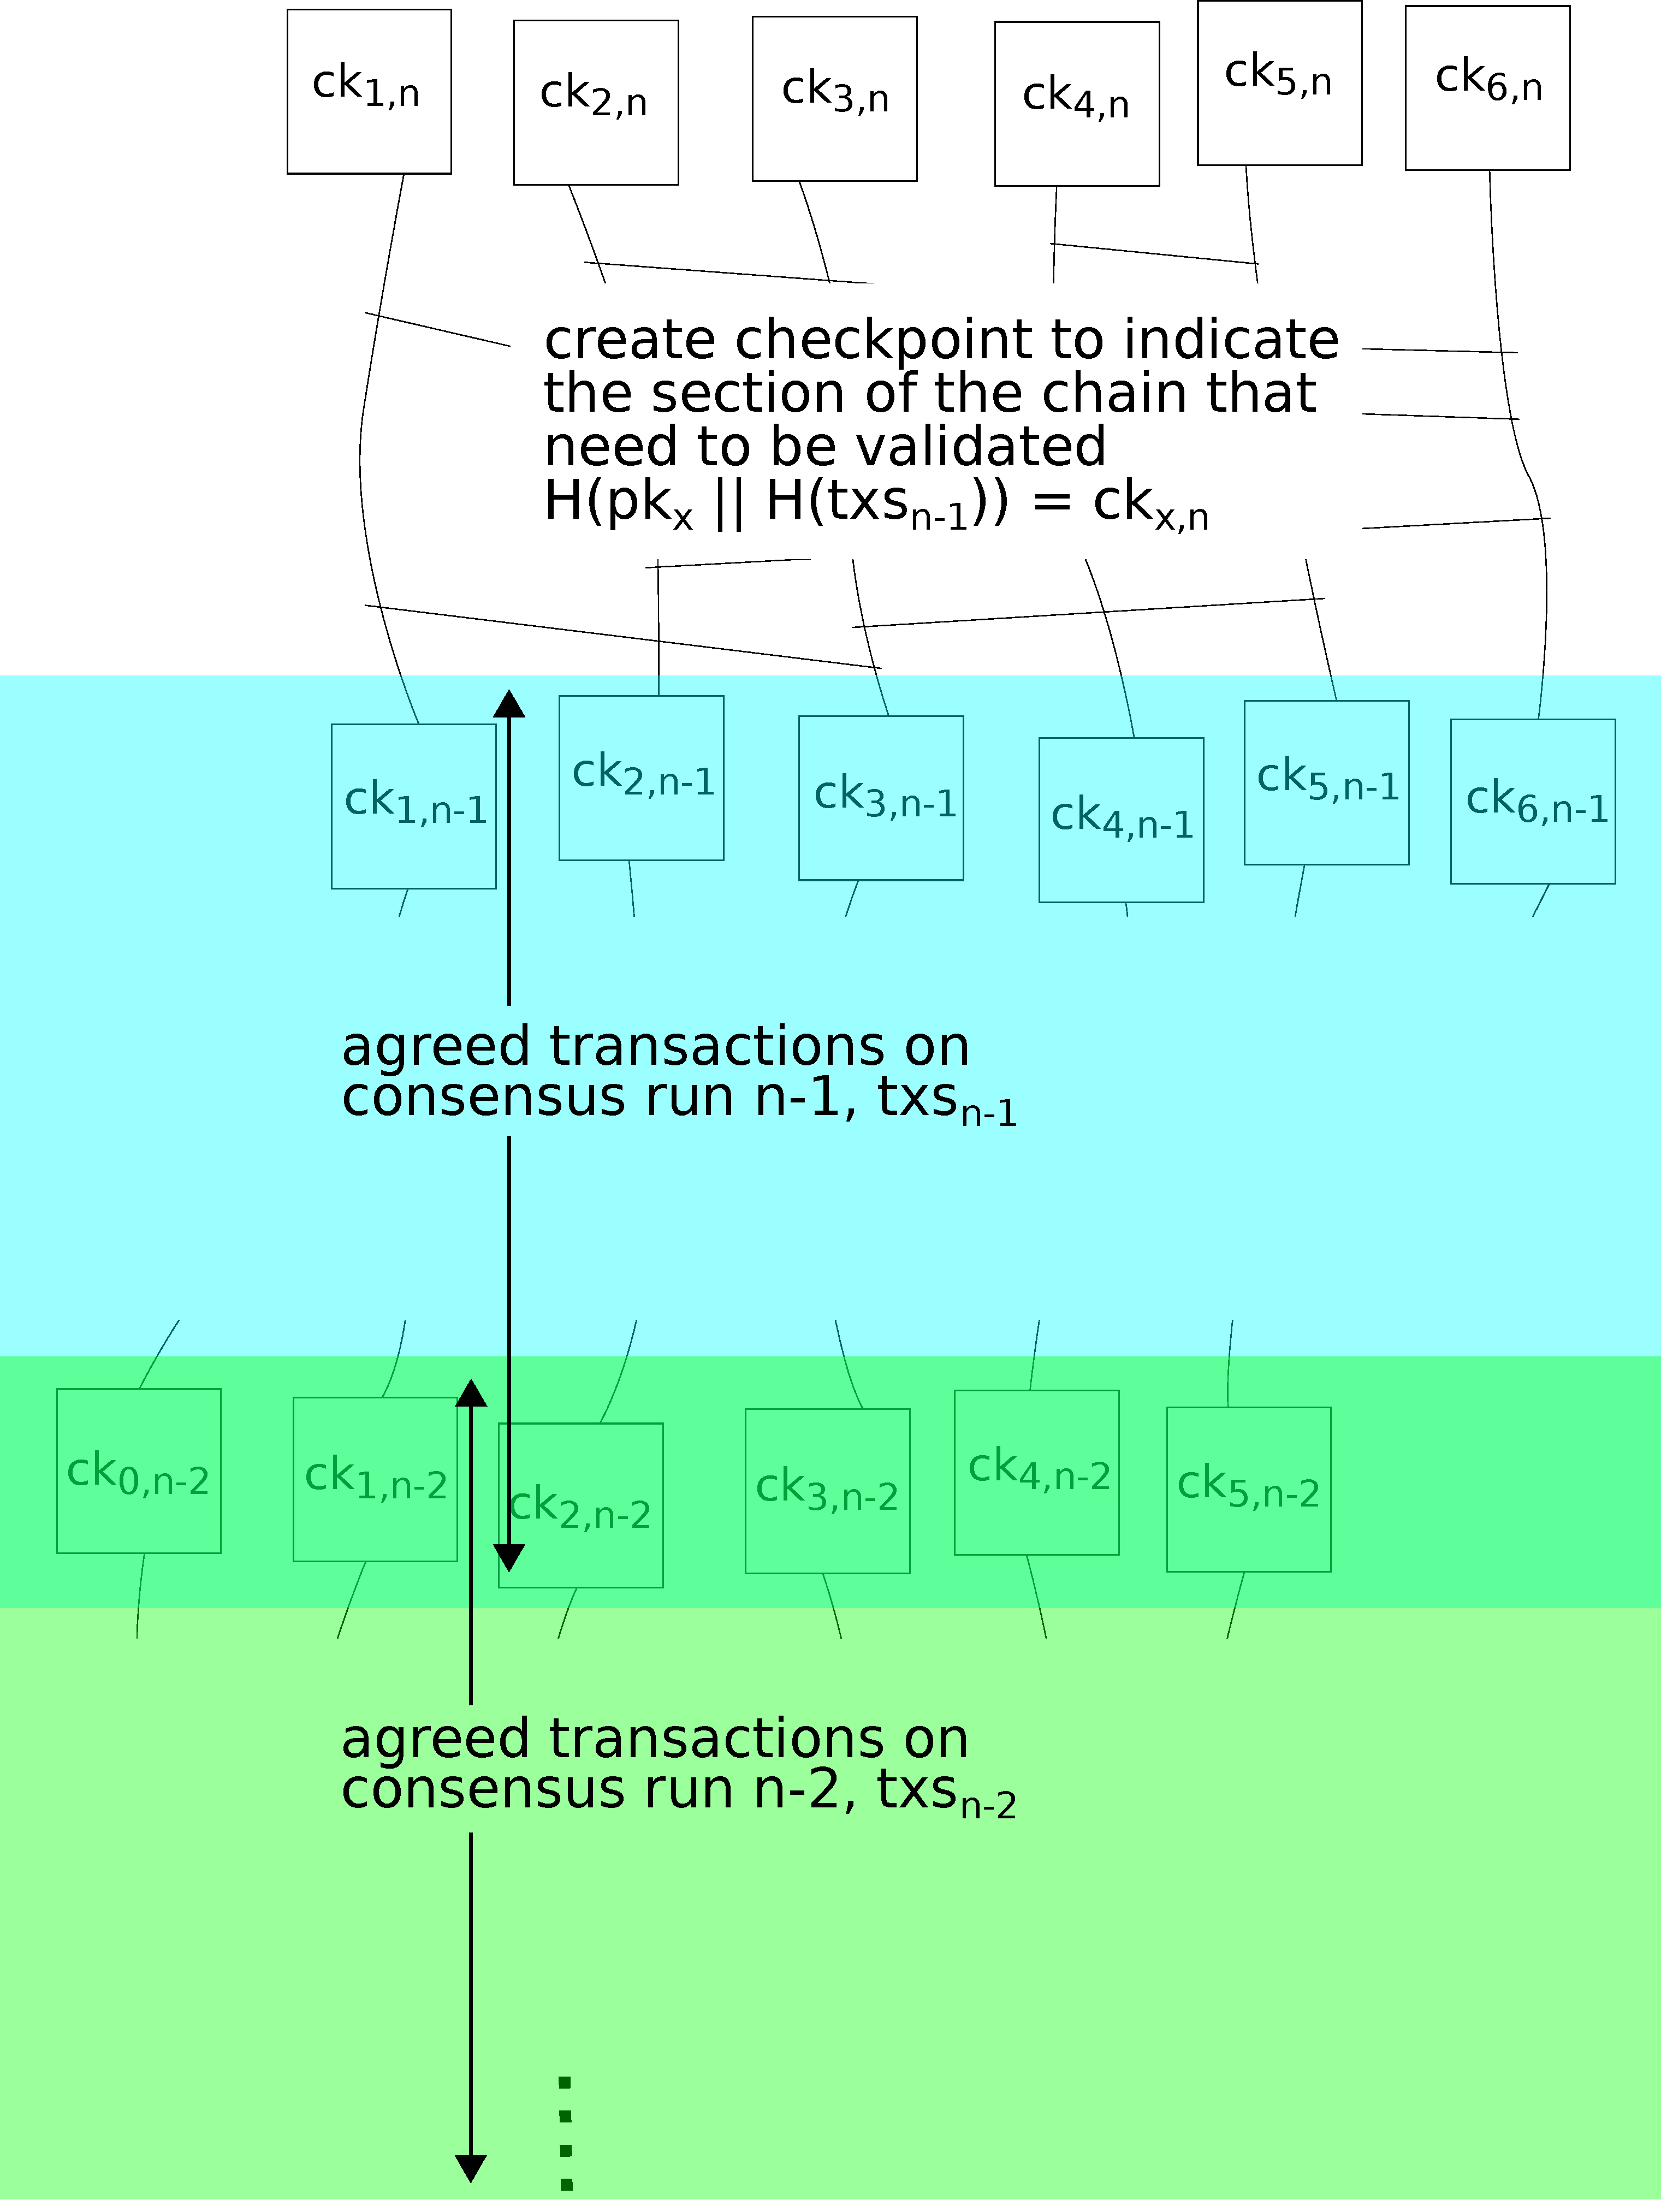
\includegraphics[width=0.7\textwidth]{figures/protocol-setup}
	\caption{In the setup phase, nodes obtains the new set of validated
      transaction from the validators and generate checkpoint blocks (top of the
      figure).}
    \label{fig:protocol-setup}
\end{figure}

\subsection{Group consensus phase}
Every node (validator or not) belong to a \emph{consensus group} (again we
assume this is known). Validators that belong to the same consensus group is
called a \emph{validator group}.

Nodes send their unvalidated chain to their respective validator groups. The
validator collect those chains for a fixed amount of time and then rejects any
new chains. Next, the validator groups perform a BFT consensus algorithm (e.g.
PBFT~\cite{castro1999practical}) and reach consensus on a set of valid
transactions. At the end of this phase, the validators in every validator group
should have a set of transactions that has reached group consensus.

If the BFT consensus algorithm is sufficient when there is only one consensus
group, then there is no need to perform the group merge phase. But most
algorithms do not scale well~\cite{vukolic2015quest}.

\subsection{Group merge phase}
Given a set of valid transaction for every validator group, we need to merge
them to achieve global consensus. We do this using a bottom-up approach, similar
to divide and conquer algorithms such as merge sort. The algorithm works in
rounds, but it does not assume a synchronous environment.

Every validator group merges with another validator group (assuming the total
number of groups is even). We assume the pairing is known just like how every
node knows the identities of the validators, but we remove the assumption later.
Validators from both groups share their validated transactions and run a BFT
algorithm to agree on the final result, which is simply the union of the two
previously validated transactions. By this point the group is merged with a new
set of validators.

The group merge phase proceeds to the next round by repeating itself until there
is only a single validator group. Groups may not finish the same round at the
same time, thus groups that finish early need to wait until its pair is ready
(by exchanging messages).
% If the pair never finishes, it implies that the majority of the nodes in the
% pair have been infiltrated by attackers. In this case, the host node

\subsection{Dissemination phase}
The validator in the final round publishes the set of validated transactions
(possibly using BitTorrent) and the Merkle hash of the validated transactions
(possibly in a hierarchical way). They also create a self-transaction in their
own chain that contains the Merkle hash.

\subsection{Consensus group formation}\label{sec:consensus-group}
Until now we always assumed the consensus groups and validator groups are known,
in this and the subsequent sections we describe a novel technique to perform
group formation.

Group formation is a hard problem in distributed systems because it is
essentially a consensus problem---every node need to know the group membership
information of every other node. Even worse, running a BFT algorithm may not be
possible in this case because we have dynamic group sizes.

Our novel idea is to piggyback on the latest consensus result. Every node knows
the latest consensus result $txs_{n-1}$ (if they don't they can ask the
validators) or the Merkle hash of it $H(txs_{n-1})$, then they perform some
deterministic computation to find the luck value
$$l_{x,n-1} = H(H(txs_{n-1}) || pk_{x})$$
for every node that participated in $txs_{n-1}$. The consensus group for $x$ in
consensus run $n$ on round $k$ (initially at 0) is then
$$
g_{x,n,k} = l_{x, n-1} \mod 2^{m-k},
$$
where $m$ can be for example 8, it depends on the estimated number of users
and the target consensus group size.

Computing the cryptographic hash for every node in the set may become expensive,
and poor clients may fail to do it in time. We can work around this by having
the validators send the membership information to all members of their consensus
group.

\subsection{Validator group formation}\label{sec:validator-group}
Validators all belong to a consensus group, but only lucky nodes are allowed to
be validators. To find the luckiness, we use the same luck value $l_{x,n-1}$,
and check for the inequality
$$
l_{x, n-1} < D,
$$
where $D$ is the difficulty value and a system parameter (undecided). Nodes that
satisfies the inequality are considered lucky.

Recall that validator groups merge and create a new set of valid transactions.
So the validator groups need to answer the following two questions.
\begin{enumerate}
\item Which other validator group to pair up (this information need to be
  symmetrical)?
  \item Who are the new validators in the merged validator group?
\end{enumerate}
The answer for (1) is encoded in $g_{x,n,k}$, namely $g_{x,n,k} = g_{x,n,k-1}
\mod 2^{m-k}$. The information for (2) is the first $c$ validators ordered by
their luck, where $c$ is a system parameter (undecided).

In essence, every node runs a deterministic algorithm on the latest consensus
result to determine the consensus group, validator group, etc. for the next
consensus run. With this, we circumvent the permissionless problem with
classical BFT algorithms.

\subsection{Bootstrapping}\label{sec:bootstrapping}
The protocol need to be bootstrapped, in this section we provide a possible
method.

From the genesis block up until some consensus run $n$, there would be no
validator group formation, all validation are performed by servers run by the
developer. This property can be implemented in the client software (similar to
how Bitcoin performs protocol upgrades). From consensus run $n+1$ and onwards,
the validator groups begin to form and the system begins to run the full
bottom-up consensus protocol.

\section{Choosing the right BFT consensus algorithm}
PBFT~\cite{castro1999practical} assumes weak synchrony. It uses a primary node
to initiate the algorithm which may not fit nicely with our model. But it is
somewhat successful in Tendermint and Hyperledger (citation and verification
needed).

HoneyBadgerBFT~\cite{miller2016honey} and Cachin's secure broadcast
protocol~\cite{cachin2001secure} may suite our needs more, but further
investigation is needed. The advantage of these two protocols over PBFT is that
they work in the asynchronous environment.

\section{Limitations, Discussion and Questions}
\begin{itemize}
\item What's the mechanisms for publishing double-spends?
\item Doesn't prevent spam, so DoS is possible. But we can work around this by
  ignoring spammy nodes.
\item If there is stake in the system, we can use it to elect validator, this
  would prevent the sybil attack. But I argue sybil attack is application
  dependent.
\item No incentive in this system, but again it's application specific.
\item If a node is offline for some time, it will not be in any consensus group.
  To join a consensus group, it must make a transaction to a node that is in a
  consensus group.
\item Not all the validators are online (chrun), but we can model it using the
  Sleep consensus model~\cite{bentov2016sleepy}.
\item This model does not require a single connected component. 
\item I personally don't see a lot of benefit with the idea of spontaneously
  growing the set of valid transaction by traversing the DAG, in the end
  everything must be validated anyway, and I don't see any major advantages of
  that technique. It also must assume single connected component, where as this
  approach does not.
\end{itemize}

\subsection{Merging consensus groups does not guarantee BFT with a probability
  of 1}
Our assumption is that $n > 3f$, this can be alternatively written as $n = 3f +
1$, for the set of all validators. Suppose the validators are put into $c$
groups and each group has $\frac{n}{c}$ validators. The bottom-up consensus
protocol requires every validator group to reach consensus, thus if a group has
$\frac{n}{3c}$ or more Byzantine nodes, then the group cannot reach consensus.
We claim if Byzantine nodes can freely choose validator groups, then they can
prevent consensus for $c-1$ groups.

We can write
$$
f = \frac{n-1}{3} = x \frac{n}{3c},
$$
where $x$ is the number validator groups that the Byzantine group can
infiltrate. Suppose $x = c$, then
$$f = \frac{n-1}{3} < c \frac{n}{3c} = \frac{n}{3},$$
this implies that the number Byzantine nodes is insufficient to infiltrate all
$c$ groups. Now suppose $x = c - 1$, then we claim
$$f > (c-1) \frac{n}{3c}$$
for $n > c$. This is easy to see
\begin{align*}
  f = \frac{n-1}{3} &> (c-1)\frac{n}{3c} \\
  n - 1 &> n\frac{c-1}{c} \\
  \frac{n-1}{n} &> \frac{c-1}{c} \\
  n &> c.
\end{align*}
This result implies that there is a sufficient number of Byzantine nodes to
infiltrate $c - 1$ groups.

While this disheartening, there may be a few ways to improve on it or look at it
in a different light.
\begin{itemize}
\item The analysis assumes that the Byzantine nodes can choose which group to
  join, but in our protocol they cannot. Thus the aforementioned result is the
  worst case scenario.
\item Perhaps we do not aim BFT with a probability of 1, but try to achieve BFT
  with a sufficiently high probability. Randomisation of group membership helps
  here.
\item Does our approach break down when a consensus run is infiltrated by
  Byzantine nodes? Can we recover afterwards? My intuition says yes, because
  honest nodes will always detect malicious transactions due to the TrustChain
  structure. Thus they will not accept the ``validated'' transactions from the
  Byzantine nodes, and they can publish a proof of malicious transaction in
  future consensus runs.
\item There is always one consensus group that is not infiltrated, can it do
  something about the situation?
\item The bottom-up approach is aimed to make BFT consensus algorithms scale. In
  some applications it may be sufficient even without the bottom-up approach
  (HoneyBadgerBFT can handle thousands of transactions on 64
  nodes~\cite{miller2016honey}).
\item The comparison (theoretical and practical) between bottom-up and
  non-bottom-up would make an interesting thesis topic.
\end{itemize}

\subsection{Tail bounding the number of Byzantine nodes in a consensus group}
We want to answer the following question. \emph{Suppose there is an urn that has
  $N$ balls, $M = (2N+1)/3$ of them are white and $N - M$ of them are black.
  $N/c$ balls are drawn without replacement. What is the probability that the
  number of white balls drawn is lower than the expected number of white balls?}
This question maps directly to our problem of Byzantine nodes, where the urn is
the set of all validators and they form $c$ groups each of size $N/c$. The white
balls represent honest nodes and the black balls represent Byzantine nodes.

The problem is modelled by the hypergeometric distribution\footnote{This is a
  variation of the geometric distribution where the balls are picked without
  replacement.} and we can solve it using tail inequalities.

Using the notation and definition in~\cite{skala2013hypergeometric}, the tail
inequality (not necessarily tight) is given by
\[
\Pr[ i \le E[i] - tn ] \le e^{-2t^2n},
\]
where $i$ is the random variable (the number of white balls), $E[i] = n
\frac{M}{N}$ is the expected value and $n = N/c$ is the number of balls drawn.
For our problem, we are interested in the probability that the number of white
balls is lower than the expected value. Thus we can write $\Pr[i \le E[i] - 1]$,
and then
\begin{align*}
  tn &= 1 \\
  tN/c &= 1 \\
  t &= c/N.
\end{align*}
Finally we get
\begin{align*}
  \Pr[ i \le E[i] - 1] &\le e^{-2 (c/N)^2 (N/c)} \\
  \Pr[ i \le E[i] - 1] &\le e^{-2 (c/N)}
\end{align*}

To minimise the probability, we must maximise $c/N$. But $c/N < 1$, so parameter
tuning cannot help us to reach a vanishingly small probability. This may be the
nail in the coffin for the current algorithm.


\subsection{How to set the initial validator group size?}
This can be modelled as the occupancy problem.

\section{Is the traditional Byzantine Agreement too strict?}
If nodes are in agreement, they share the same state machine. But is this too
strict for our use case?

Suppose there is set of transactions $A \rightarrow B \rightarrow C \rightarrow
D$ that depend on each other. Then half of the nodes agree on a subset of those
transactions, i.e. $\{A, B, C\}$. Another half agree on all four transactions.
This is not Byzantine agreement in the traditional sense, because there does not
exist a majority that share the same state machine. But indirectly they all
agree on the set intersection. Can we build a model that support this type of
consensus?

%  LocalWords:  BFT Merkle checkpointing permissionless setup

%%% Local Variables:
%%% mode: latex
%%% TeX-master: "../thesis"
%%% End:


\clearemptydoublepage

%Choose a good bibliography style, plain would do often, but these might be nice too
%\bibliographystyle{these}
\bibliographystyle{plain}
\bibliography{references}

%% Uncomment for appendix
%\clearemptydoublepage
%
%\appendix
%\addcontentsline{toc}{chapter}{Appendix}
%
%\chapter{My First Appendix}
In this file (appendices/main.tex) you can add appendix chapters, just as you did in the thesis.tex file for the `normal' chapters.
You can also choose to include everything in this single file, whatever you prefer.

\end{document}
